\documentclass[10pt, conference, letterpaper]{IEEEtran}

\usepackage{algorithm}
\usepackage{algorithmicx}
\usepackage{algpseudocode}
\usepackage{amsfonts}
\usepackage{amsmath}
\usepackage{amssymb}
\usepackage[ansinew]{inputenc}
\usepackage{xcolor}
\usepackage{mathtools}
\usepackage{graphicx}
\usepackage{caption}
\usepackage{subcaption}
\usepackage{import}
\usepackage{multirow}
\usepackage{cite}
\usepackage[export]{adjustbox}
\usepackage{breqn}
\usepackage{mathrsfs}
\usepackage{acronym}
\usepackage{setspace}
\usepackage{bm}
\usepackage{stackengine}
\usepackage{booktabs}

\graphicspath{{./figures/}}
\setlength{\belowcaptionskip}{0mm}
\setlength{\textfloatsep}{8pt}

\newcommand{\eq}[1]{Eq.~\eqref{#1}}
\newcommand{\fig}[1]{Fig.~\ref{#1}}
\newcommand{\tab}[1]{Tab.~\ref{#1}}
\newcommand{\secref}[1]{Section~\ref{#1}}

\DeclareMathOperator*{\argmin}{arg\,min}
\DeclareMathOperator*{\argmax}{arg\,max}

\setlength{\columnsep}{0.2in}

\title{Fine-Grained Car Make Classification Using Convolutional Neural Networks with Hierarchical Multi-Task Learning}

\author{Alexandru Mihailescu\thanks{Work done for the course of Neural Networks and Deep Learning, taught by Prof. Jacopo Pegoraro and Prof. Michele Rossi at the University of Padua.}}

\IEEEoverridecommandlockouts

\begin{document}

\maketitle

\begin{abstract}
Fine-grained visual categorization of automobiles has applications in autonomous driving, intelligent transportation, surveillance, and insurance claim processing. This report compares convolutional neural network architectures for car make classification on the CompCars classification split, 30,955 images across 75 makes and 431 models. Five models are evaluated: a baseline CNN trained from scratch, ResNet50, EfficientNet-B0, ResNet50 augmented with Squeeze-and-Excitation attention, and a hierarchical multi-task network that predicts make (75 classes) and model (431 classes) from a shared backbone with dual heads. The hierarchical network is the best model, reaching 87.55\% top-1 make accuracy and 82.72\% top-1 model accuracy on the test split, which exceeds the OverFeat baseline of Yang et al. by 4.65 and 6.02 percentage points respectively; its second head costs nothing at inference. Transfer learning from ImageNet is the dominant factor: pretrained backbones reach 80\% to 88\% test accuracy against 53.08\% from scratch. SE attention adds 1.79 points over ResNet50 for 0.7M parameters, and EfficientNet-B0 reaches 86.95\% with 4.1M parameters at twice the throughput of any ResNet50 variant. Focal loss does not help despite a 120:1 class imbalance, losing 1.89 points to cross-entropy. Every model loses 10 to 22 accuracy points between the random validation split and the official test split, so validation accuracy on this benchmark is a model-selection signal and not a performance estimate.
\end{abstract}

\IEEEkeywords
Fine-Grained Classification, Convolutional Neural Networks, Transfer Learning, Attention Mechanisms, Multi-Task Learning, Vehicle Recognition.
\endIEEEkeywords

% !TEX root = report.tex

\section{Introduction}
\label{sec:introduction}

Fine-grained visual categorization (FGVC) distinguishes visually similar subcategories inside a broader category, such as separate car makes and models~\cite{Yang2015}. Unlike general object classification, it requires capturing subtle discriminative cues on objects that are nearly identical at the coarse level. Vehicle classification has direct applications in autonomous driving, traffic monitoring, law enforcement, and automated insurance assessment.

The CompCars dataset~\cite{Yang2015} contains over 136,000 web-nature images spanning 163 makes and 1,716 models. The official classification subset used here contains 30,955 images across 75 makes and 431 models. The original work reported 82.9\% make accuracy and 76.7\% model accuracy using OverFeat features with multi-view fusion. That is the reference point used throughout this report.

Five CNN architectures are evaluated on that subset. The findings are:

\begin{itemize}
    \item A hierarchical multi-task classifier that jointly predicts make (75 classes) and model (431 classes) from a shared backbone reaches 87.55\% top-1 make accuracy and 82.72\% top-1 model accuracy on the test split, exceeding the OverFeat baseline by 4.65 and 6.02 percentage points respectively.
    \item Transfer learning dominates every other design choice. Pretrained backbones reach 80\% to 88\% test accuracy; the same training recipe from scratch reaches 53.08\%.
    \item Squeeze-and-Excitation attention~\cite{Hu2018} adds 1.79 percentage points over ResNet50 with label smoothing, at a cost of 0.7M parameters.
    \item EfficientNet-B0~\cite{Tan2019} reaches 86.95\% with 4.1M parameters, beating a 24.6M-parameter ResNet50~\cite{He2016} while sustaining roughly twice its inference throughput.
    \item Focal loss~\cite{Lin2017} does not help. Despite a 120:1 class imbalance it loses 1.89 points against plain cross-entropy.
\end{itemize}

\secref{sec:related_work} reviews related work. \secref{sec:model} covers the dataset and preprocessing. \secref{sec:architectures} details the architectures. \secref{sec:learning_framework} covers losses and optimization. \secref{sec:results} presents the results and \secref{sec:conclusions} concludes.


% !TEX root = report.tex

\section{Related Work}
\label{sec:related_work}

\subsection{Fine-Grained Visual Categorization}

FGVC has been studied extensively for birds~\cite{WahCUB2002011}, aircraft, and vehicles. Early approaches relied on part-based models and hand-crafted features, and required explicit part annotations at training time. Current methods use deep CNNs with attention to localize discriminative regions without manual supervision, which improves both accuracy and scalability.

\subsection{The CompCars Dataset}

Yang et al.~\cite{Yang2015} introduced CompCars, a large-scale car dataset for fine-grained categorization and verification, with web-nature and surveillance-nature images annotated hierarchically by make, model, and year. Using OverFeat features with multi-view fusion they reported 82.9\% on make classification and 76.7\% on model classification. That result is the primary baseline here, and the hierarchical annotation is what makes the multi-task formulation of \secref{sec:architectures} possible.

\subsection{Deep CNN Architectures}

ResNet~\cite{He2016} introduced skip connections that allow very deep networks to train without gradient degradation, and the residual formulation scales to hundreds of layers while remaining trainable.

EfficientNet~\cite{Tan2019} uses compound scaling to jointly optimize depth, width, and resolution through neural architecture search. It reaches a better accuracy-to-parameter ratio, with EfficientNet-B0 matching ResNet50 accuracy using 6$\times$ fewer parameters. Both architectures gain substantially from transfer learning on domain-specific tasks with limited data.

\subsection{Attention Mechanisms}

Squeeze-and-Excitation Networks~\cite{Hu2018} apply channel attention: global average pooling followed by fully-connected layers that recalibrate channel-wise feature responses. Modelling channel interdependence explicitly lets a network emphasize informative channels and suppress the rest. For fine-grained classification this is directly useful, since the discriminative evidence sits in narrow visual details such as grilles, headlights, and body contours.

\subsection{Transfer Learning}

Pretraining on ImageNet~\cite{Deng2009} and fine-tuning on the target domain is standard for recognition tasks with limited training data. The learned features transfer across domains and supply both a better initialization and implicit regularization. Differential learning rates (lower for pretrained layers, higher for new classifier heads) preserve the learned representation while the task-specific layers adapt.


% !TEX root = report.tex

\section{Dataset and Preprocessing}
\label{sec:model}

\subsection{Dataset Overview}

The CompCars classification subset contains 30,955 images: 16,016 for training and 14,939 for testing, across 75 makes and 431 models. \tab{tab:dataset} reports the split statistics.

\begin{table}[ht]
\centering
\caption{CompCars Classification Subset Statistics}
\label{tab:dataset}
\small
\setlength{\tabcolsep}{4pt}
\begin{tabular}{lcc}
\toprule
\textbf{Statistic} & \textbf{Train} & \textbf{Test} \\
\midrule
Images & 16,016 & 14,939 \\
Makes / Models & 75 / 431 & 75 / 431 \\
Min / Max samples per make & 10 / 1,201 & 9 / 1,125 \\
Mean $\pm$ std samples per make & 213.5 $\pm$ 228.7 & 199.2 $\pm$ 215.5 \\
Min / Max samples per model & 10 / 143 & 8 / 140 \\
Mean $\pm$ std samples per model & 37.2 $\pm$ 21.4 & 34.7 $\pm$ 21.3 \\
\bottomrule
\end{tabular}
\end{table}

Two properties of the data drive the rest of the design. First, the make labels are severely imbalanced, with a 120:1 ratio between the largest and smallest training class (1,201 against 10 samples). The model labels are only mildly imbalanced at 14.3:1. Second, the images vary widely in viewpoint, lighting, and background clutter, so the features have to be robust to nuisance variation rather than merely discriminative on canonical shots.

A 10\% stratified validation split was carved out of the training data for scheduler control and early stopping, preserving the class proportions.

\subsection{Image Preprocessing}

All images were pre-resized to 256$\times$256 pixels to fix input dimensions and cut data-loading cost.

\textbf{Training augmentation.} Random resized crops (224$\times$224, scale 0.8 to 1.0), horizontal flips at probability 0.5, color jitter (brightness, contrast, saturation $\pm$0.2), and random rotation ($\pm$15\textdegree).

\textbf{Evaluation preprocessing.} Deterministic center crop to 224$\times$224 with no augmentation, for validation and test.

\textbf{Normalization.} ImageNet statistics (mean [0.485, 0.456, 0.406], std [0.229, 0.224, 0.225]) so that inputs match the distribution the pretrained backbones expect.

\section{Model Architectures}
\label{sec:architectures}

Five architectures were evaluated, spanning a from-scratch baseline, two standard pretrained backbones, an attention-augmented backbone, and a multi-task variant.

\subsection{SimpleCNN Baseline}

A 4-block VGG-style network (64$\rightarrow$128$\rightarrow$256$\rightarrow$512 channels) with batch normalization, global average pooling, and a dropout plus linear classifier, trained entirely from scratch (\fig{fig:simplecnn}). It holds 1.6M parameters and fixes the lower bound against which transfer learning is measured.

\begin{figure}[ht]
\centering
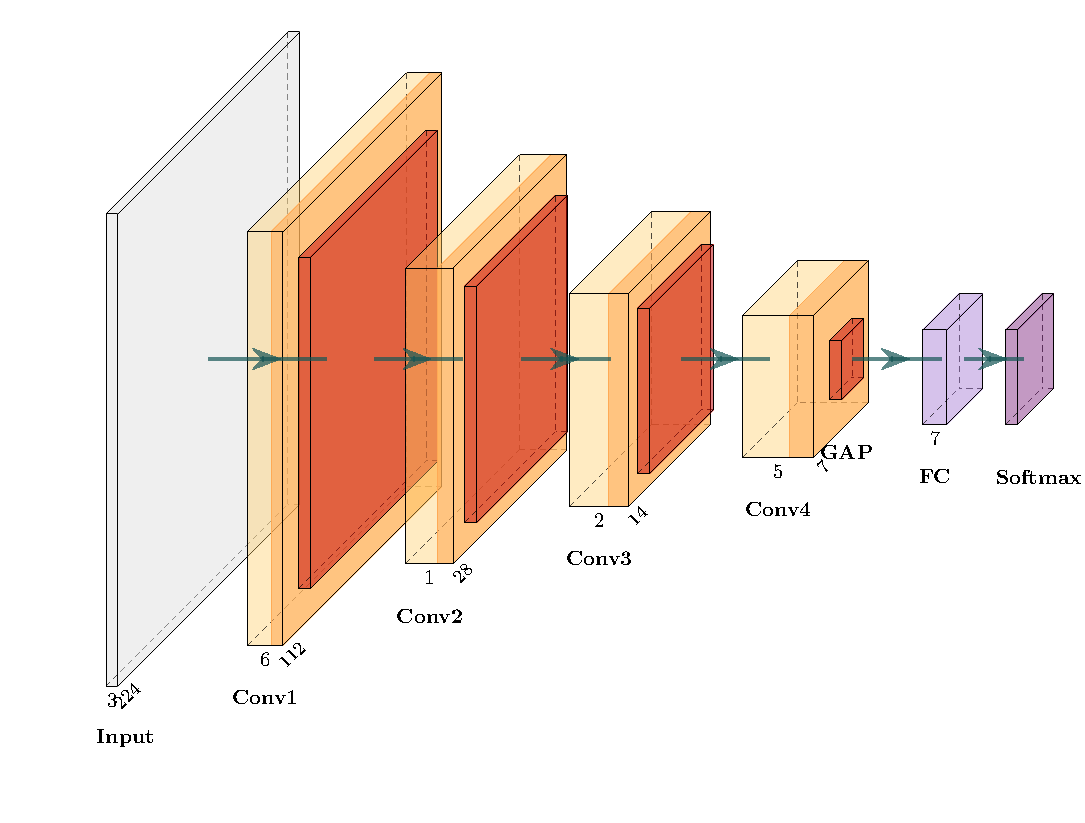
\includegraphics[width=\columnwidth]{figures/simplecnn.pdf}
\caption{SimpleCNN architecture: 4-block VGG-style network trained from scratch.}
\label{fig:simplecnn}
\end{figure}

\subsection{ResNet50}

ResNet50~\cite{He2016} with ImageNet-pretrained weights (\fig{fig:resnet50}). The original classifier is replaced by a two-layer head (2048$\rightarrow$512$\rightarrow$75) with dropout at 0.5 and 0.3, for 24.6M parameters in total. All layers are trainable.

\begin{figure}[ht]
\centering
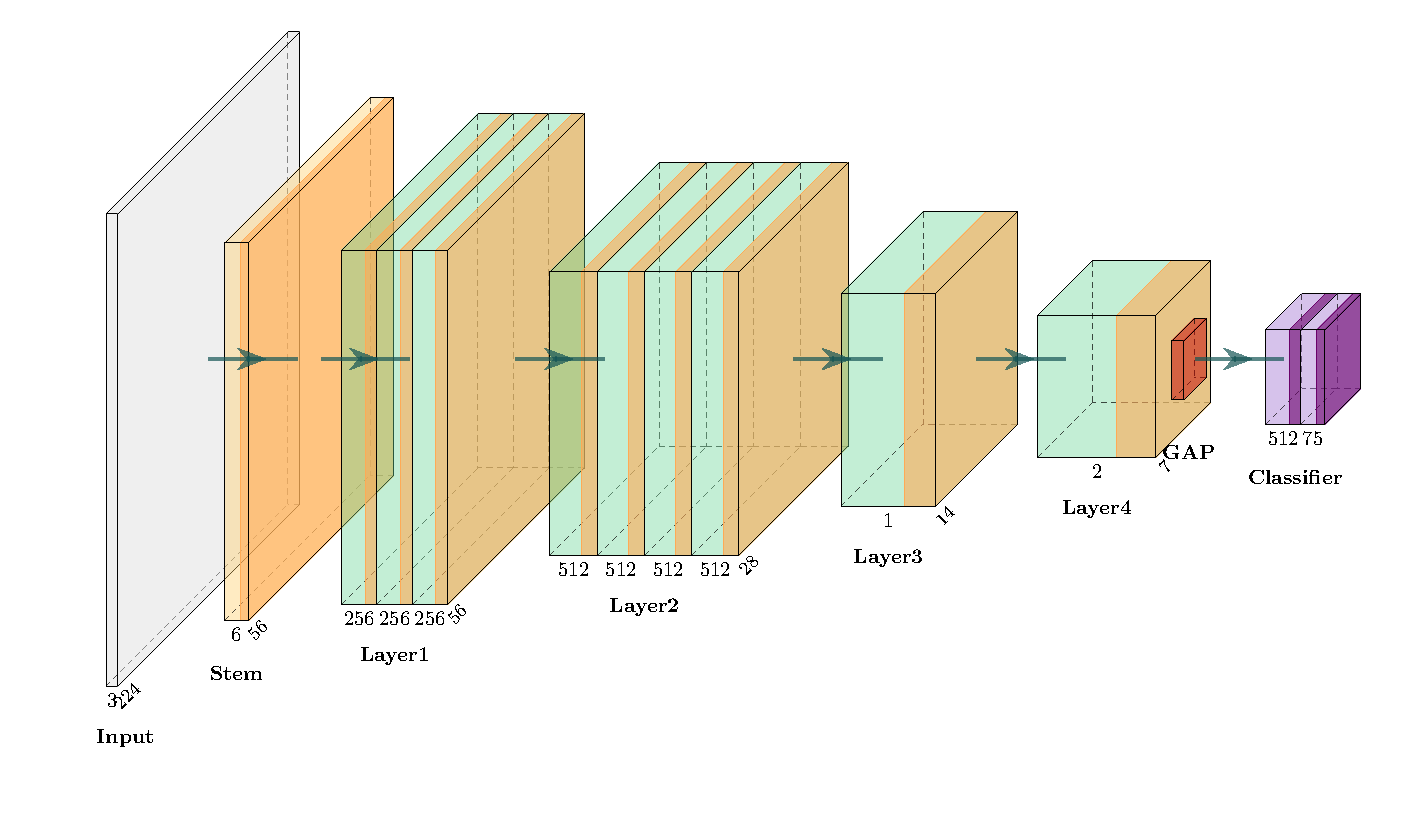
\includegraphics[width=\columnwidth]{figures/resnet50.pdf}
\caption{ResNet50 architecture with custom classifier head.}
\label{fig:resnet50}
\end{figure}

\subsection{EfficientNet-B0}

EfficientNet-B0~\cite{Tan2019} uses compound scaling over depth, width, and resolution (\fig{fig:efficientnet}). It is built from MBConv blocks with depthwise separable convolutions, Swish activations, and squeeze-and-excitation attention already inside each block. With a single dropout plus linear head it holds 4.1M parameters, 6$\times$ fewer than ResNet50.

\begin{figure}[ht]
\centering
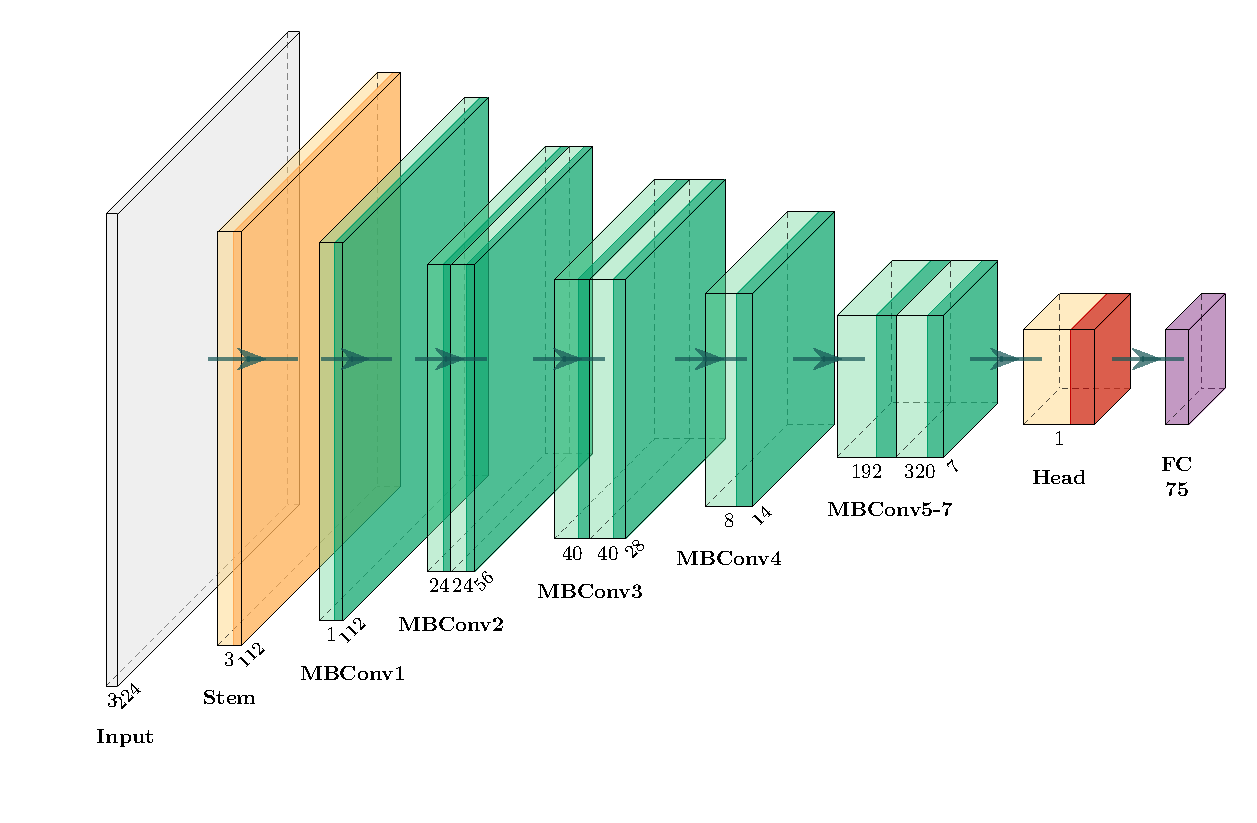
\includegraphics[width=\columnwidth]{figures/efficientnet.pdf}
\caption{EfficientNet-B0 architecture with MBConv blocks and SE attention.}
\label{fig:efficientnet}
\end{figure}

\subsection{ResNet50 with SE Attention}

ResNet50-SE inserts a Squeeze-and-Excitation block after each of the four residual stages (\fig{fig:resnet50se}). Each block performs global average pooling to squeeze the spatial dimensions, two fully-connected layers with reduction ratio 16 to model channel dependence, and sigmoid-gated rescaling of the original features. The four blocks add roughly 0.7M parameters (8K, 32K, 131K, and 524K for the 256, 512, 1024, and 2048 channel stages). The head is a single dropout plus linear layer, which is why the total (24.36M) sits slightly below the two-layer-head ResNet50 (24.60M) despite the extra attention parameters.

\begin{figure}[ht]
\centering
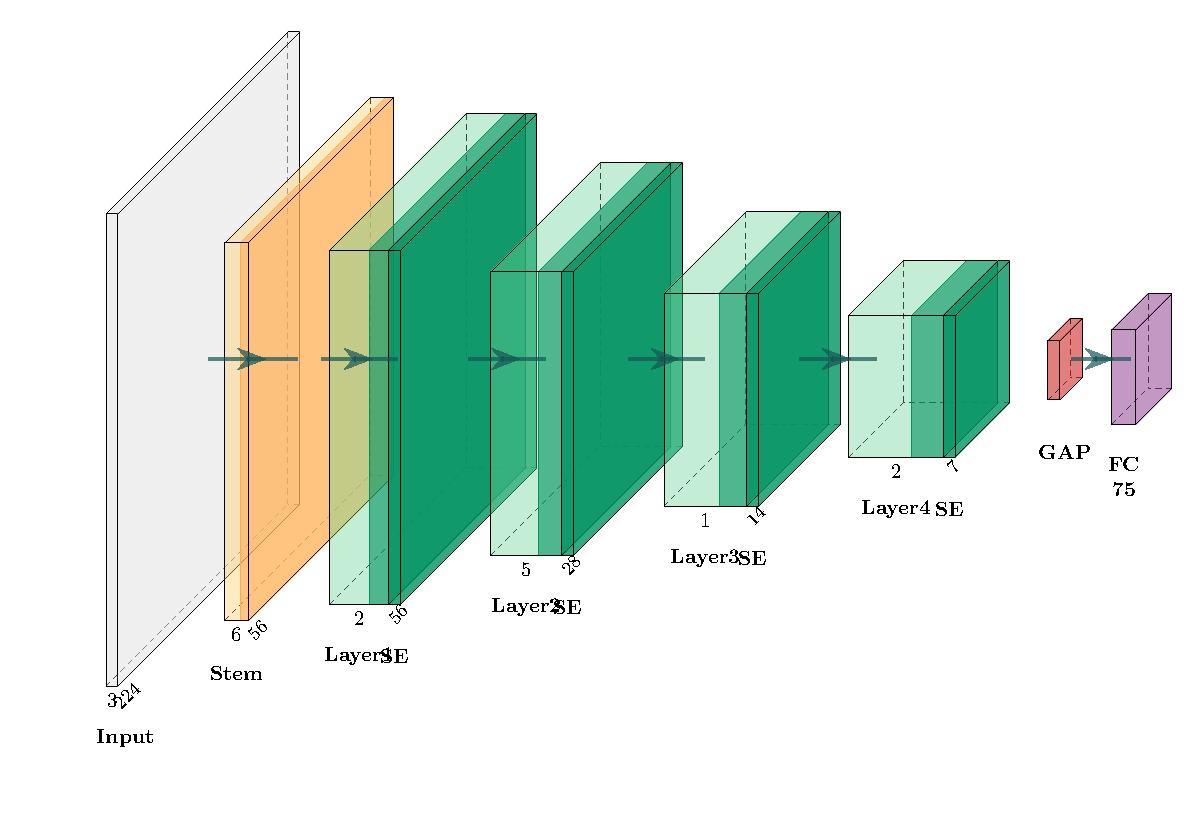
\includegraphics[width=\columnwidth]{figures/resnet50_se.pdf}
\caption{ResNet50-SE architecture with SE attention blocks after each stage.}
\label{fig:resnet50se}
\end{figure}

\subsection{Hierarchical Multi-Task Classifier}

The hierarchical classifier exploits the coarse-to-fine structure of the annotation (\fig{fig:hierarchical}). A shared ResNet50 backbone feeds two parallel two-layer heads: make (2048$\rightarrow$512$\rightarrow$75) and model (2048$\rightarrow$512$\rightarrow$431). Both heads see the same 2048-dimensional pooled feature. The auxiliary model task forces the backbone to retain the fine detail that separates variants inside a make, which the make head then reuses. Total parameters: 25.9M (23.5M backbone, 1.09M make head, 1.27M model head).

\begin{figure}[ht]
\centering
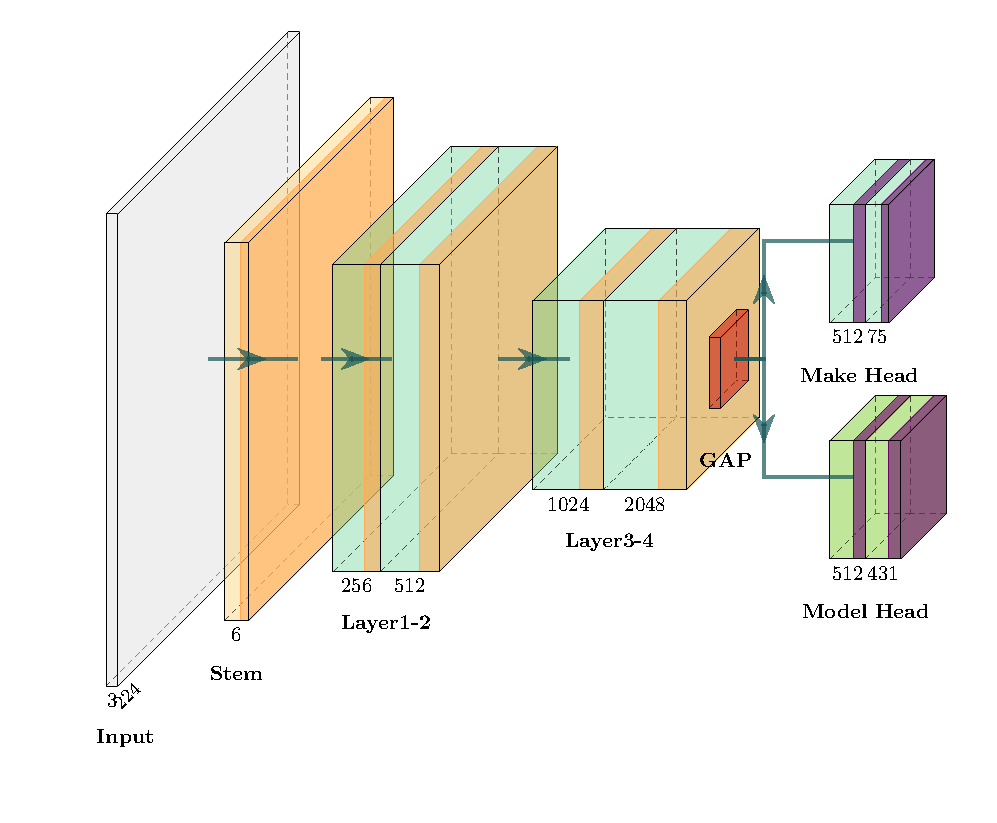
\includegraphics[width=\columnwidth]{figures/hierarchical.pdf}
\caption{Hierarchical classifier with shared backbone and dual classification heads.}
\label{fig:hierarchical}
\end{figure}

\section{Training Methodology}
\label{sec:learning_framework}

\subsection{Loss Functions}

\textbf{Cross-entropy.} The baseline. All misclassifications weighted equally regardless of class frequency.

\textbf{Focal loss.} Focal loss~\cite{Lin2017} with $\gamma$=2 down-weights easy examples so that gradient mass concentrates on hard ones. It is the standard answer to class imbalance and is included precisely to test that claim on this dataset.

\textbf{Label smoothing.} Cross-entropy with smoothing 0.1, which spreads a small probability mass over non-target classes and penalizes overconfidence.

\textbf{Hierarchical loss.} The multi-task model minimizes
\begin{equation}
\mathcal{L} = \alpha \cdot \mathcal{L}_{\text{make}} + (1-\alpha) \cdot \mathcal{L}_{\text{model}},
\label{eq:hier}
\end{equation}
with $\alpha$=0.3, so 70\% of the loss weight sits on the harder 431-class model task. Both terms use cross-entropy with label smoothing 0.1.

\subsection{Optimization Strategy}

AdamW with differential learning rates: $10^{-4}$ for pretrained backbones and $10^{-3}$ for the randomly initialized heads. The backbone keeps its ImageNet features while the heads adapt quickly.

Training ran for 100 epochs at batch size 32, weight decay $10^{-4}$, and gradient clipping at max norm 1.0. A ReduceLROnPlateau scheduler halved the learning rate after 3 epochs without validation improvement; early stopping with patience 5 restored the best validation checkpoint. Mixed precision (AMP) cut memory use by roughly 40\% on the 12GB RTX 3060 used for all runs. For the hierarchical model the scheduler and early stopping track make accuracy.

\subsection{Hyperparameter Summary}

\tab{tab:hyperparams} lists the configuration, identical across all experiments except for the loss.

\begin{table}[ht]
\centering
\caption{Training Hyperparameters}
\label{tab:hyperparams}
\begin{tabular}{ll}
\toprule
\textbf{Parameter} & \textbf{Value} \\
\midrule
Batch size & 32 \\
Backbone learning rate & $10^{-4}$ \\
Classifier learning rate & $10^{-3}$ \\
Weight decay & $10^{-4}$ \\
Epochs & 100 \\
Scheduler patience & 3 \\
Early stopping patience & 5 \\
Label smoothing & 0.1 \\
Hierarchical $\alpha$ & 0.3 \\
\bottomrule
\end{tabular}
\end{table}


% !TEX root = report.tex

\section{Experimental Results}
\label{sec:results}

\subsection{Overall Performance}

The hierarchical classifier wins on every test metric: 87.55\% top-1, 94.77\% top-5, and 0.870 macro F1. It exceeds the OverFeat baseline~\cite{Yang2015} by 4.65 percentage points. \tab{tab:main_results} gives the full comparison and \fig{fig:accuracy_comparison} plots top-1 against top-5 accuracy.

\begin{table}[ht]
\centering
\caption{Test Set Results for Make Classification (75 Classes). Precision, Recall and F1 are macro-averaged.}
\label{tab:main_results}
\small
\setlength{\tabcolsep}{3.5pt}
\begin{tabular}{lcccccc}
\toprule
\textbf{Model} & \textbf{Params} & \textbf{Top-1} & \textbf{Top-5} & \textbf{Prec.} & \textbf{Rec.} & \textbf{F1} \\
\midrule
SimpleCNN & 1.6M & 53.08 & 77.12 & 0.572 & 0.426 & 0.459 \\
ResNet50 (CE) & 24.6M & 82.28 & 91.88 & 0.839 & 0.769 & 0.789 \\
ResNet50 (Focal) & 24.6M & 80.39 & 91.12 & 0.830 & 0.742 & 0.763 \\
ResNet50 (LS) & 24.6M & 82.69 & 88.47 & 0.794 & 0.814 & 0.770 \\
EfficientNet-B0 & 4.1M & 86.95 & 94.50 & 0.897 & 0.833 & 0.853 \\
ResNet50-SE & 24.4M & 84.48 & 93.78 & 0.911 & 0.821 & 0.853 \\
\textbf{Hierarchical} & 25.9M & \textbf{87.55} & \textbf{94.77} & 0.910 & 0.849 & \textbf{0.870} \\
\midrule
OverFeat~\cite{Yang2015} & n/a & 82.90 & n/a & n/a & n/a & n/a \\
\bottomrule
\end{tabular}
\end{table}

\begin{figure}[ht]
\centering
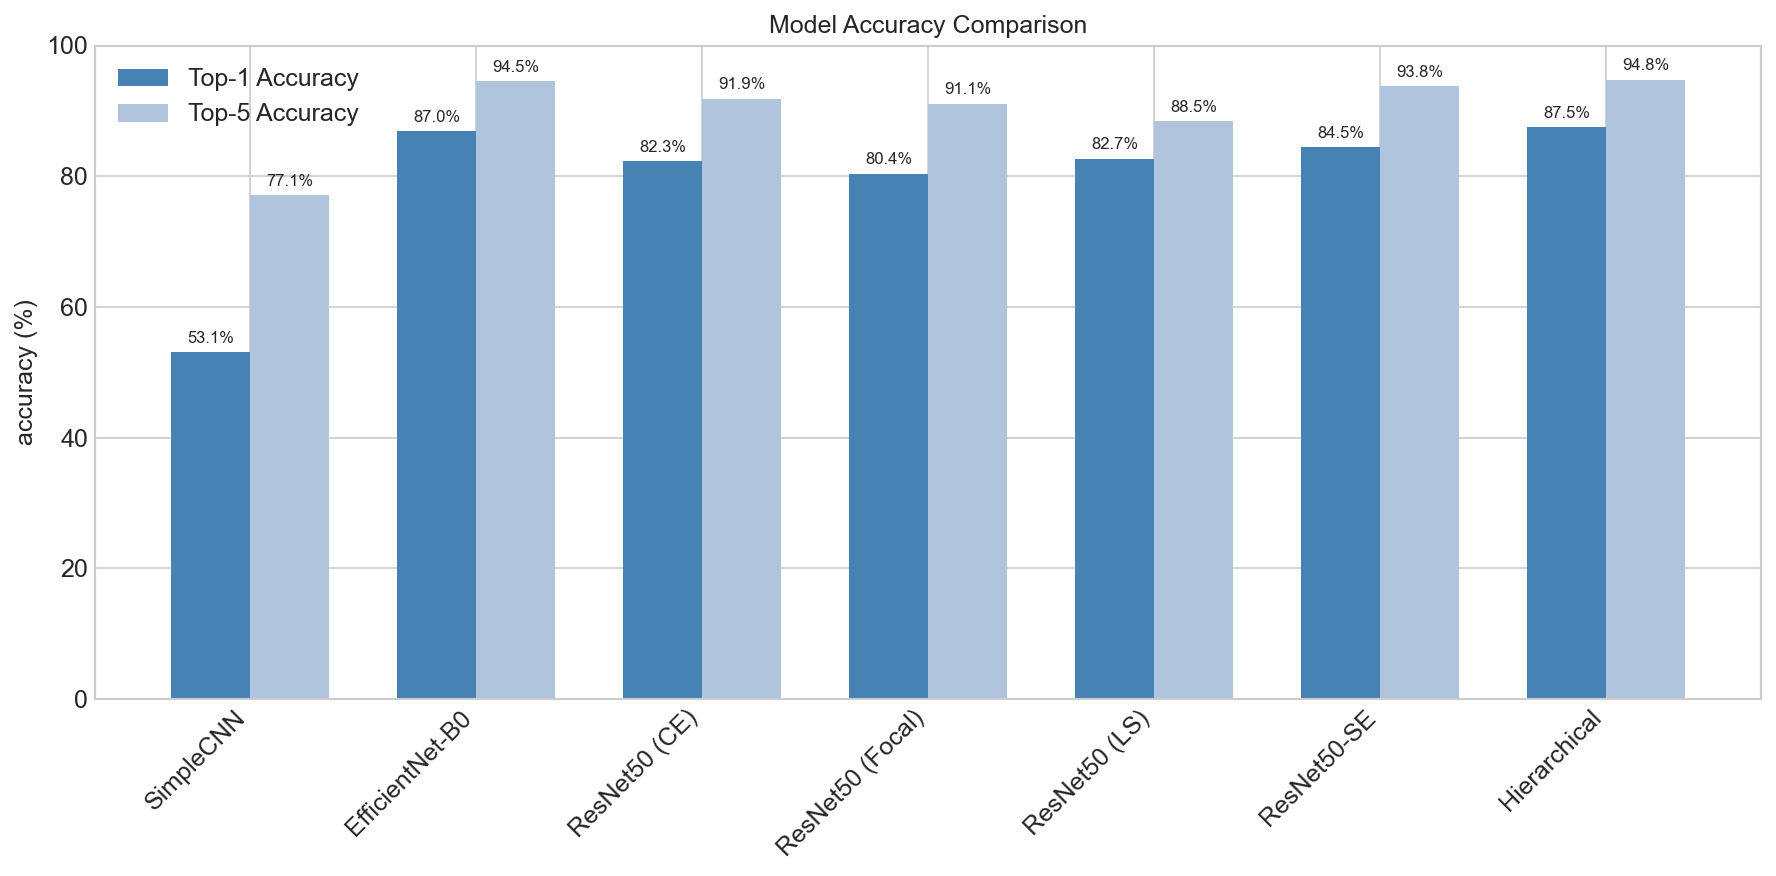
\includegraphics[width=\columnwidth]{figures/accuracy_comparison.png}
\caption{Top-1 and Top-5 accuracy comparison across all models.}
\label{fig:accuracy_comparison}
\end{figure}

Macro recall is consistently the weakest of the three averaged metrics, and it separates the models more than top-1 does. ResNet50-SE and the hierarchical model reach almost identical macro precision (0.911 against 0.910) but differ by 2.8 points of recall (0.821 against 0.849). The models are conservative on rare classes rather than wrong about them, which the per-class analysis below confirms.

\subsection{Impact of Transfer Learning}

Transfer learning is the single largest effect in the study. SimpleCNN, trained from scratch under the same schedule, reaches 53.08\% test accuracy against 80.39\% to 86.95\% for the pretrained backbones, a spread of 27 to 34 percentage points. Its macro F1 (0.459) is barely half that of any pretrained model.

The gap shows in the training dynamics as well. SimpleCNN converges more slowly and overfits harder, and its validation accuracy stalls at 74.78\% while training accuracy climbs to 85.80\%. Without ImageNet features the network has to learn edges, textures, and shape priors from 16k images, and it does not have enough data to do so.

\subsection{Architecture Comparison}

\subsubsection{Attention}

SE blocks lift ResNet50 with label smoothing from 82.69\% to 84.48\%, a gain of 1.79 points for 0.7M attention parameters. The larger gain is in macro precision, from 0.794 to 0.911, and in top-5 accuracy, from 88.47\% to 93.78\%. Channel recalibration mostly removes confident wrong answers rather than adding new correct ones.

\subsubsection{Parameter Efficiency}

EfficientNet-B0 reaches 86.95\% with 4.1M parameters. It beats the 24.6M-parameter ResNet50 (LS) by 4.26 points using 6$\times$ fewer parameters, and comes within 0.6 points of the hierarchical model at one sixth of its size. \fig{fig:acc_vs_params} shows the trade-off. Depthwise separable convolutions, compound scaling, and the SE attention built into every MBConv block all contribute; note that the built-in attention is consistent with the independent gain measured for ResNet50-SE.

\begin{figure}[ht]
\centering
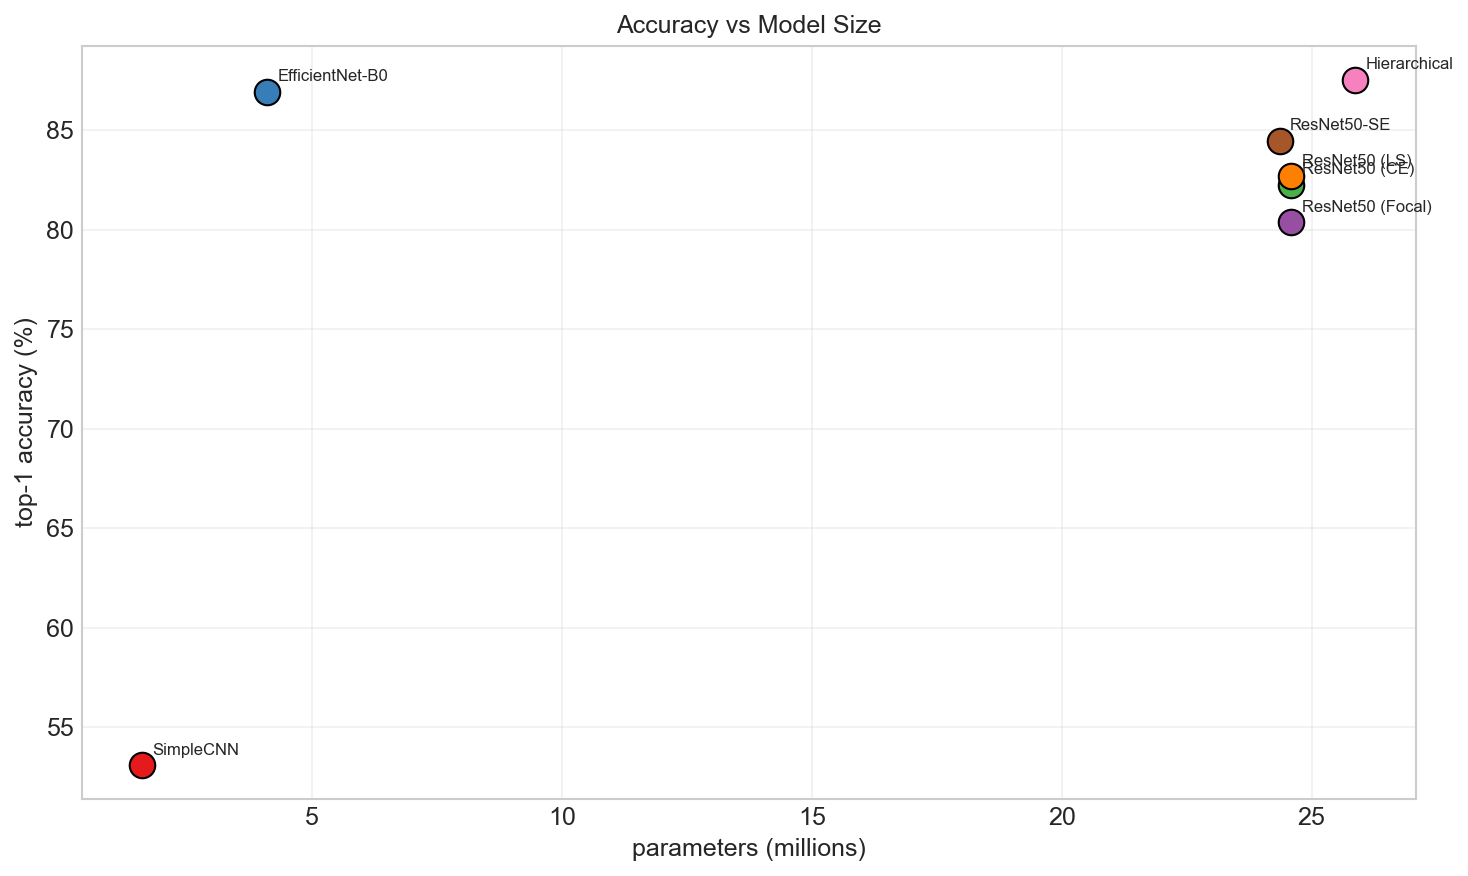
\includegraphics[width=\columnwidth]{figures/acc_vs_params.png}
\caption{Test accuracy against model size. EfficientNet-B0 is the efficiency winner.}
\label{fig:acc_vs_params}
\end{figure}

\subsection{Inference Cost}

Parameter count alone does not settle deployment. \tab{tab:timing} reports measured inference over the full 14,939-image test set at batch size 32 on an RTX 3060.

\begin{table}[ht]
\centering
\caption{Inference Cost (RTX 3060, batch size 32, 14,939 images)}
\label{tab:timing}
\begin{tabular}{lccc}
\toprule
\textbf{Model} & \textbf{Params} & \textbf{ms/image} & \textbf{Images/s} \\
\midrule
SimpleCNN & 1.60M & 0.58 & 1734 \\
EfficientNet-B0 & 4.10M & 1.18 & 844 \\
ResNet50 (CE) & 24.60M & 2.43 & 411 \\
ResNet50 (Focal) & 24.60M & 2.44 & 410 \\
ResNet50 (LS) & 24.60M & 2.46 & 406 \\
ResNet50-SE & 24.36M & 2.54 & 394 \\
Hierarchical & 25.87M & 2.38 & 420 \\
\bottomrule
\end{tabular}
\end{table}

EfficientNet-B0 sustains 844 images per second, roughly double any ResNet50 variant, while giving up 0.6 accuracy points to the best model. The SE blocks cost about 3.5\% throughput against ResNet50 (LS) for their 1.79-point gain. The second head of the hierarchical model is free at inference: 420 images per second, statistically indistinguishable from plain ResNet50, because the heads are trivial next to the shared backbone. If the make prediction is all that is needed, the model head can simply be discarded.

\subsection{Loss Function Comparison}

\tab{tab:loss_comparison} compares losses on ResNet50 with everything else held fixed. Focal loss ($\gamma$=2) loses 1.89 points to cross-entropy despite the 120:1 imbalance it is designed for. Label smoothing gains 0.41 points on top-1 but loses 3.41 points of top-5 accuracy (88.47\% against 91.88\%), so it is not a clear win either.

\begin{table}[ht]
\centering
\caption{Loss Function Comparison (ResNet50)}
\label{tab:loss_comparison}
\small
\setlength{\tabcolsep}{4pt}
\begin{tabular}{lcccc}
\toprule
\textbf{Loss Function} & \textbf{Val Acc} & \textbf{Test Top-1} & \textbf{Test Top-5} & \textbf{$\Delta$ Top-1} \\
\midrule
Cross-Entropy & 97.75\% & 82.28\% & 91.88\% & baseline \\
Focal ($\gamma$=2) & 96.69\% & 80.39\% & 91.12\% & -1.89 \\
Label Smoothing & 97.57\% & 82.69\% & 88.47\% & +0.41 \\
\bottomrule
\end{tabular}
\end{table}

The choice of loss is worth at most 2 points here, an order of magnitude less than the choice of backbone initialization. Focal loss down-weights the easy majority of examples, and on a dataset where the head classes are large but not pathological that mostly removes useful gradient signal. Imbalance is not the binding constraint on this task; the discriminability of the classes is.

\subsection{Training Dynamics}

\fig{fig:val_accuracy} and \fig{fig:val_loss} show validation accuracy and loss. All pretrained models are within a point of their peak by roughly epoch 20. Best validation accuracies: hierarchical 98.94\%, ResNet50-SE 98.00\%, EfficientNet-B0 and ResNet50 (CE) 97.75\%, ResNet50 (LS) 97.57\%, ResNet50 (Focal) 96.69\%, SimpleCNN 74.78\%.

Wall-clock training time for the full 100-epoch schedule ranged from 22 minutes (SimpleCNN) through 53 minutes (EfficientNet-B0) to roughly 1h22m for the ResNet50 family and 1h24m for the hierarchical model. The second head adds no meaningful training cost either.

\begin{figure}[ht]
\centering
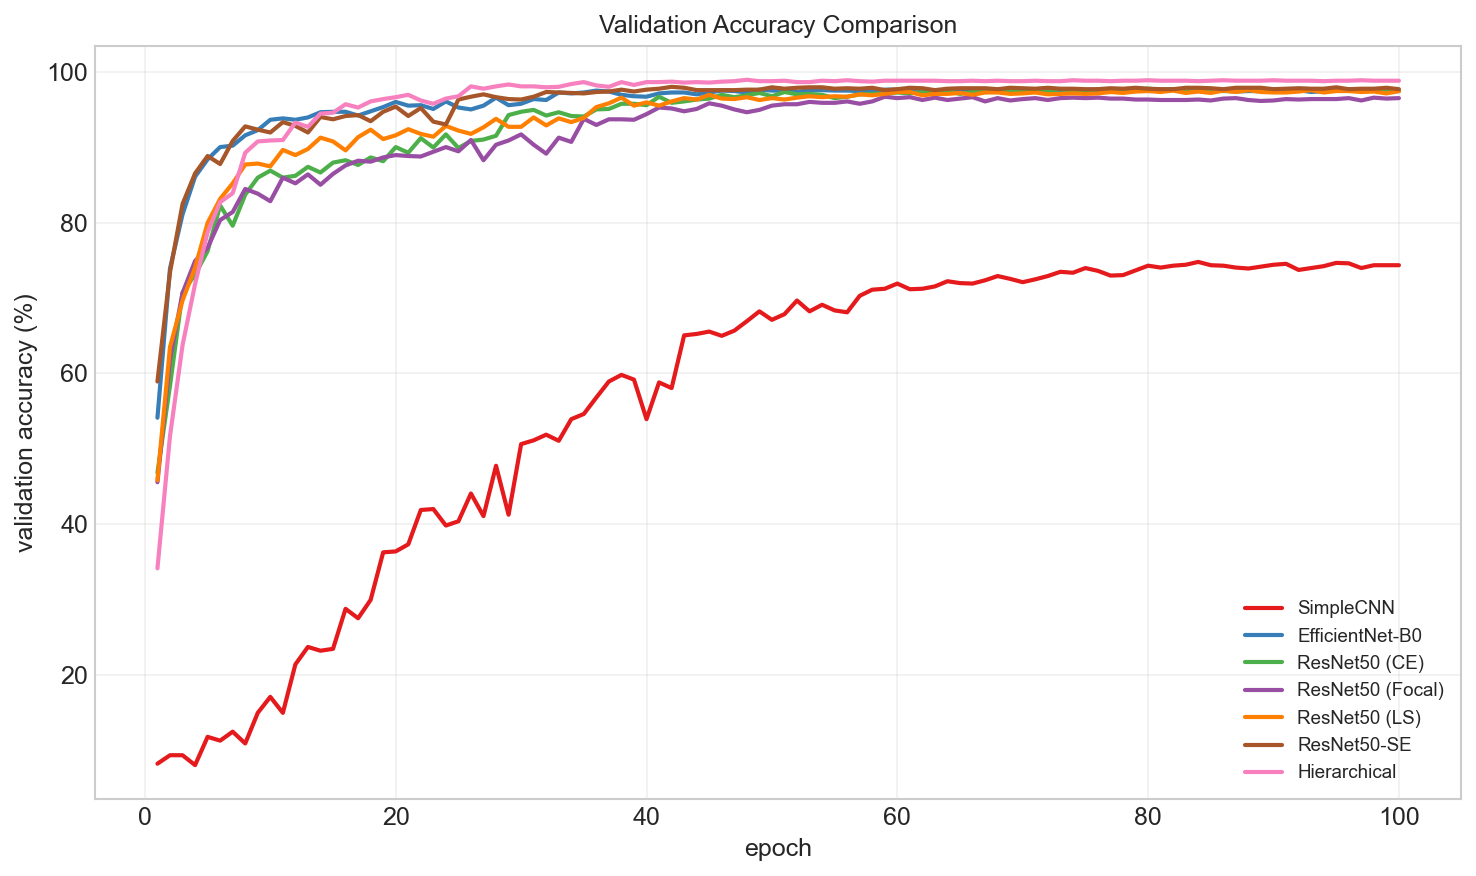
\includegraphics[width=\columnwidth]{figures/val_accuracy_overlay.png}
\caption{Validation accuracy during training for all models.}
\label{fig:val_accuracy}
\end{figure}

\begin{figure}[ht]
\centering
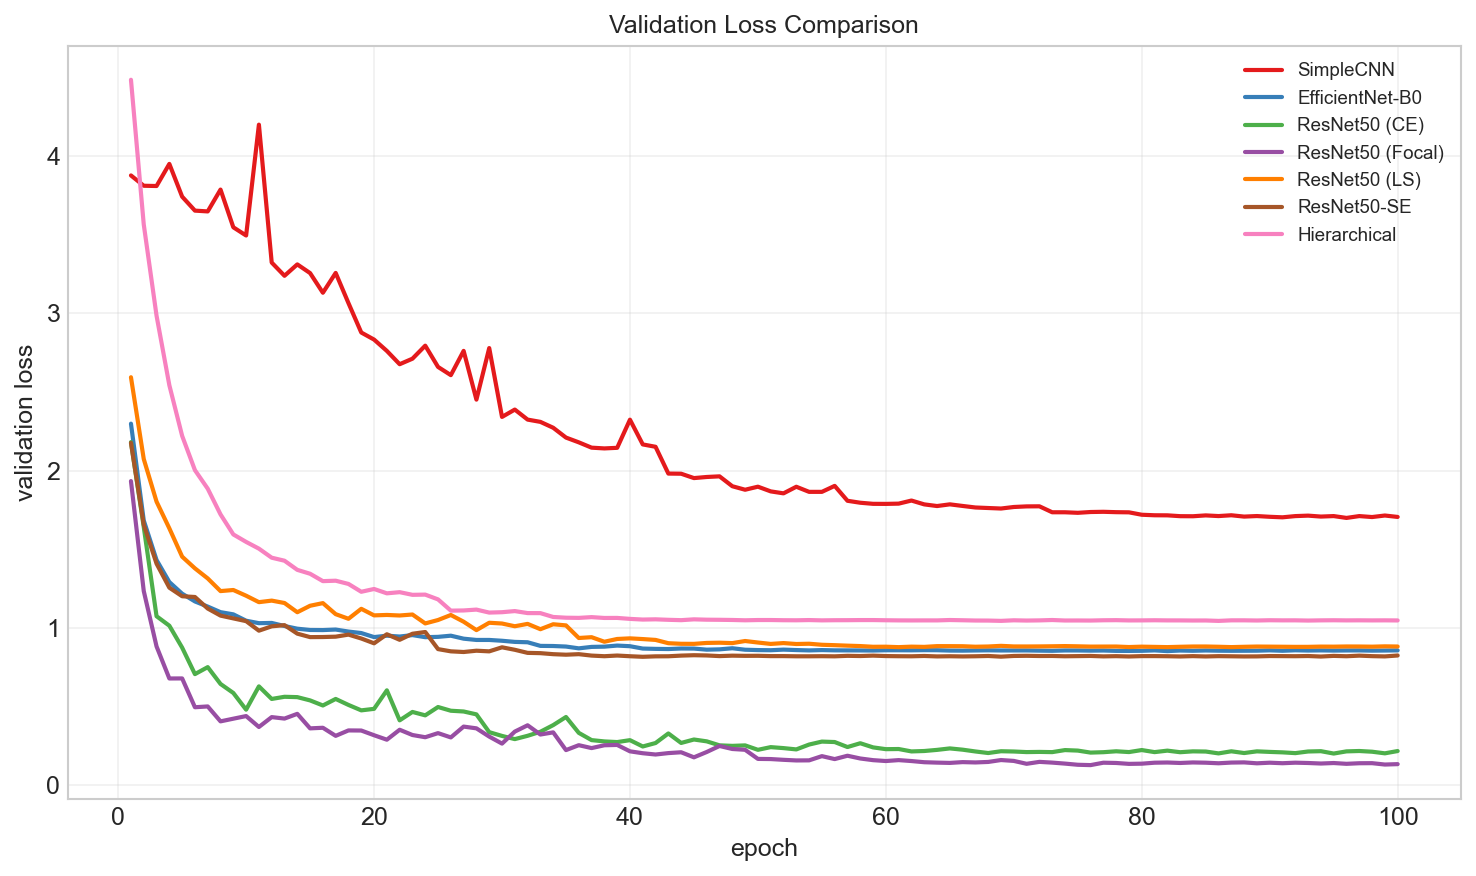
\includegraphics[width=\columnwidth]{figures/val_loss_overlay.png}
\caption{Validation loss during training for all models.}
\label{fig:val_loss}
\end{figure}

\subsection{Generalization Analysis}

Two gaps matter and they tell different stories. \tab{tab:gen_gap} reports both: the train-to-validation gap averaged over the last 10 epochs, and the validation-to-test gap at the best checkpoint. \fig{fig:gen_gap} shows the first throughout training.

\begin{table}[ht]
\centering
\caption{Generalization Gaps}
\label{tab:gen_gap}
\begin{tabular}{lccc}
\toprule
\textbf{Model} & \textbf{Train-Val} & \textbf{Best Val} & \textbf{Val-Test} \\
 & \textbf{(last 10 ep.)} & & \textbf{gap} \\
\midrule
SimpleCNN & 11.48\% & 74.78\% & 21.70\% \\
EfficientNet-B0 & 2.47\% & 97.75\% & 10.80\% \\
ResNet50 (CE) & 2.38\% & 97.75\% & 15.47\% \\
ResNet50 (Focal) & 3.52\% & 96.69\% & 16.30\% \\
ResNet50 (LS) & 2.62\% & 97.57\% & 14.88\% \\
ResNet50-SE & 2.22\% & 98.00\% & 13.52\% \\
\textbf{Hierarchical} & \textbf{1.18\%} & 98.94\% & \textbf{11.39\%} \\
\bottomrule
\end{tabular}
\end{table}

\begin{figure}[ht]
\centering
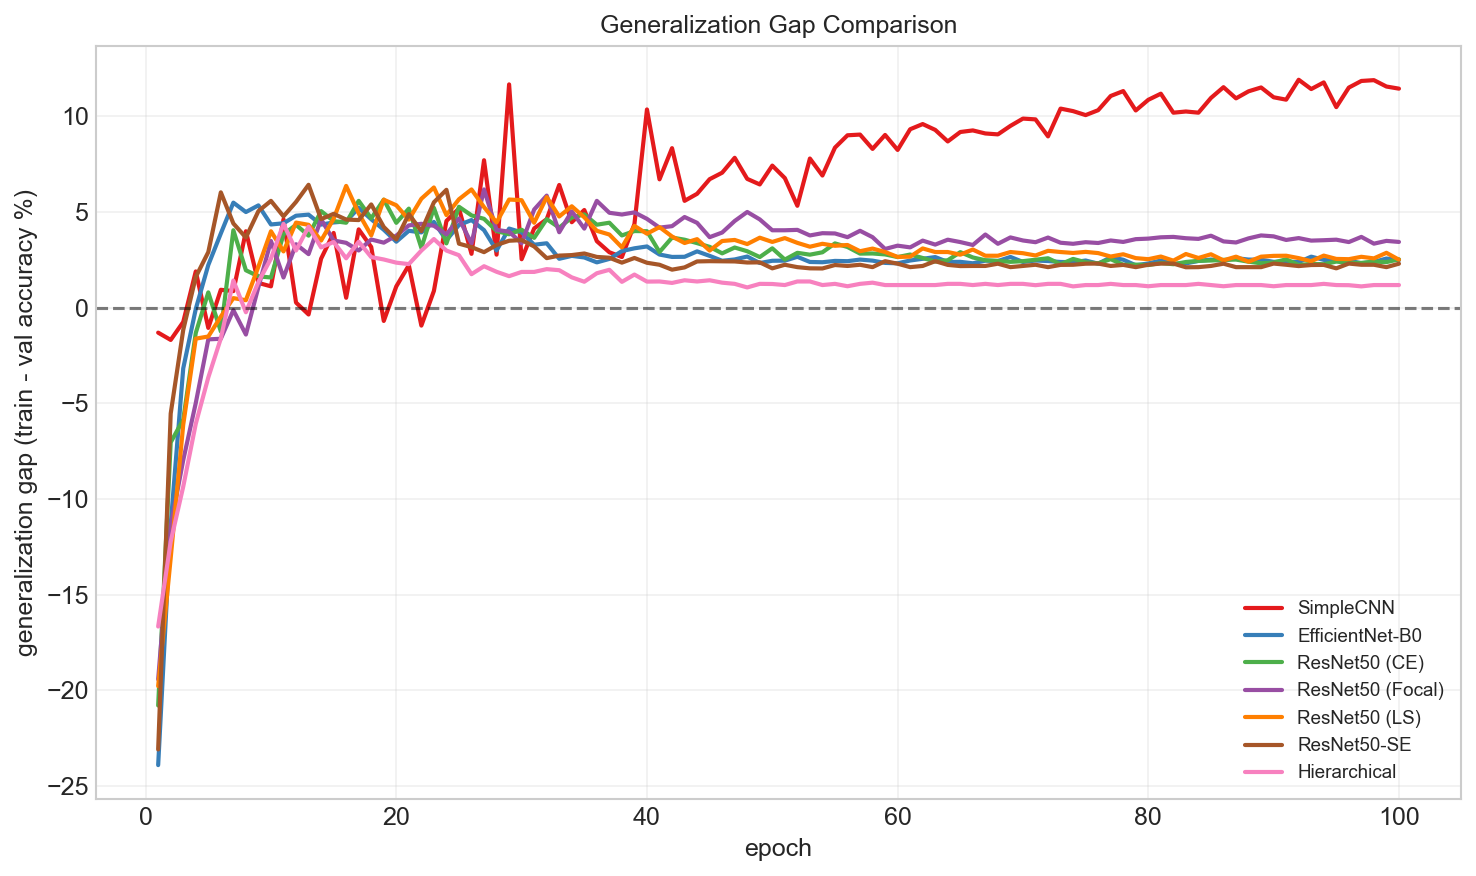
\includegraphics[width=\columnwidth]{figures/generalization_gap_overlay.png}
\caption{Train-to-validation accuracy gap throughout training. SimpleCNN diverges; the pretrained models stay flat.}
\label{fig:gen_gap}
\end{figure}

SimpleCNN's train-to-validation gap grows monotonically to 11.48\%: training accuracy keeps rising while validation accuracy flattens after roughly epoch 30. That is textbook memorization on insufficient data.

The pretrained models all sit between 1.18\% and 3.52\%, so by the train-to-validation measure they look well regularized. The validation-to-test gap contradicts that. Every model loses 10 to 22 points moving from validation to test. This is the most important negative result in the study and it is a property of the data, not of the models: the validation split is a random 10\% of the training images, so it shares photo sources, sessions, and backgrounds with the training set, while the official test split does not. Validation accuracy on this dataset is not a usable estimate of test accuracy, only a usable signal for model selection.

The ranking of the val-test gap is still informative. The hierarchical model (11.39\%) and EfficientNet-B0 (10.80\%) leak least; focal loss leaks most among the pretrained models (16.30\%).

\subsection{Per-Class Behaviour}

Aggregate accuracy hides where the errors sit. On the hierarchical model's make head, per-class F1 correlates with class size but weakly: mean F1 is 0.853 for the 23 makes with fewer than 50 test images, 0.873 for the 22 makes between 50 and 199, and 0.883 for the 30 makes with 200 or more. Nine makes fall below 0.80 F1 and seven reach 0.95 or above.

The failure mode is recall, not precision. The worst class has precision 1.00 and recall 0.39: when the model names it, it is right, but it names it rarely. The largest class in the test set (1,125 images) shows the opposite profile, precision 0.70 against recall 0.97, absorbing predictions that belong elsewhere.

That asymmetry is visible in \tab{tab:confusions}, which lists the top confusion pairs per model. Volkswagen is the sink: it is the predicted label in 7 of the hierarchical model's 10 worst confusion pairs, and 15.9\% of all Skoda test images are called Volkswagen by EfficientNet-B0 (8.8\% by the hierarchical model). This is not a modelling artefact. Skoda is a Volkswagen Group marque and shares platforms and styling language with it, and Volkswagen is the largest class in the dataset, so the prior and the visual evidence point the same way. The other recurring pairs (Zhonghua, Geely, Buck, GreatWall, Jianghuai into Volkswagen) are Chinese makes whose designs of that era borrowed heavily from the Volkswagen visual idiom.

\begin{table}[ht]
\centering
\caption{Top Confusion Pairs, Hierarchical Model}
\label{tab:confusions}
\begin{tabular}{llcc}
\toprule
\textbf{True} & \textbf{Predicted} & \textbf{Count} & \textbf{\% of true class} \\
\midrule
Skoda & Volkswagen & 25 & 8.8 \\
Zhonghua & Volkswagen & 16 & 7.1 \\
Buck & Volkswagen & 11 & 2.5 \\
Geely & Volkswagen & 9 & 4.9 \\
BYD & Haima & 9 & 4.3 \\
Citroen & Volkswagen & 9 & 2.6 \\
Volkswagen & Audi & 8 & 0.7 \\
Benz & Volkswagen & 8 & 1.3 \\
Jianghuai & Volkswagen & 8 & 3.3 \\
GreatWall & Volkswagen & 8 & 4.2 \\
\bottomrule
\end{tabular}
\end{table}

The single most extreme case in the study is EfficientNet-B0 calling 66.7\% of Brabus images Benz. Brabus is a Mercedes-Benz tuner, so those images are Mercedes bodies. The label is correct and the model is not seeing anything the pixels do not contain. This is a limit of make classification from a single image, not a fixable error.

\subsection{Hierarchical Model Analysis}

The multi-task model is the only one evaluated on both tasks. \tab{tab:hier} reports both heads on the test set.

\begin{table}[ht]
\centering
\caption{Hierarchical Model, Both Heads (Test Set)}
\label{tab:hier}
\begin{tabular}{lccc}
\toprule
\textbf{Head} & \textbf{Top-1} & \textbf{Top-5} & \textbf{Macro F1} \\
\midrule
Make (75 classes) & 87.55\% & 94.77\% & 0.870 \\
Model (431 classes) & 82.72\% & 91.80\% & 0.819 \\
\midrule
OverFeat make~\cite{Yang2015} & 82.90\% & n/a & n/a \\
OverFeat model~\cite{Yang2015} & 76.70\% & n/a & n/a \\
\bottomrule
\end{tabular}
\end{table}

The 431-class model head reaches 82.72\% top-1, which exceeds the OverFeat model-classification baseline (76.7\%) by 6.02 points, a larger margin than on the make task. A single network therefore beats the reference on both levels of the hierarchy at once.

The two heads fail together. Of the 2,582 test images where the model head is wrong, 60.0\% also have the make wrong. Conversely, of the 1,860 images where the make head is wrong, the model head still gets the exact car model right 16.8\% of the time, which means the shared features carry model identity that the make head fails to exploit on those images. The errors are correlated but not identical, which is exactly the condition under which the auxiliary task supplies useful gradient rather than a duplicate of the primary one.

The regularization effect is measurable. The hierarchical model has the lowest train-to-validation gap (1.18\% against 2.22\% for the next best) and the second-lowest val-test gap, while carrying the most parameters of any model tested. Forcing the backbone to also separate 431 models leaves it less free to memorize the 75-way make task.

\emph{Correction to a common reading of these numbers.} The validation figures for the hierarchical model (98.94\% make, 95.51\% model) are not test figures and should not be quoted as such. Test performance is 87.55\% and 82.72\%. The gap between the two is the val-test leak discussed above.

\subsection{Comparison to Baseline}

The hierarchical model exceeds OverFeat by 4.65 points on make and 6.02 points on model. The improvement is attributable to four things, in rough order of contribution:

\begin{enumerate}
    \item Residual architectures and stronger ImageNet pretraining, which the transfer-learning ablation shows to be worth 27 to 34 points on their own.
    \item The multi-task formulation, worth 4.86 points over the ResNet50 (LS) single-task model with the same backbone.
    \item Attention, worth 1.79 points in isolation.
    \item Training technique (AdamW, differential learning rates, label smoothing, AMP), worth under 1 point measurably.
\end{enumerate}


% !TEX root = report.tex

\section{Conclusion}
\label{sec:conclusions}

The hierarchical multi-task classifier is the best model on this benchmark: 87.55\% top-1 make accuracy and 82.72\% top-1 model accuracy on the CompCars test split, beating the OverFeat baseline by 4.65 and 6.02 percentage points. It also generalizes best, with the lowest train-to-validation gap of any model tested, and its second head costs nothing at inference.

\subsection{Findings}

\begin{itemize}
    \item \textbf{Transfer learning dominates.} Pretrained backbones beat the same recipe from scratch by 27 to 34 points. No other choice in this study comes within an order of magnitude of that effect.
    \item \textbf{Multi-task learning is a regularizer.} Adding the 431-class model head to a ResNet50 backbone raises make accuracy by 4.86 points over the single-task equivalent and cuts the train-to-validation gap from 2.62\% to 1.18\%.
    \item \textbf{Attention pays for itself.} SE blocks add 1.79 points for 0.7M parameters and 3.5\% throughput.
    \item \textbf{Small models win on cost.} EfficientNet-B0 gives up 0.6 points to the best model while using 6$\times$ fewer parameters and running at twice the throughput of any ResNet50 variant.
    \item \textbf{Focal loss does not fix this imbalance.} It loses 1.89 points to cross-entropy despite a 120:1 make imbalance. Class imbalance is not the binding constraint here.
    \item \textbf{Validation accuracy is not test accuracy.} Every model loses 10 to 22 points across that boundary, because the validation split is a random slice of the training images while the official test split is not. Validation is usable for model selection and useless as a performance estimate.
\end{itemize}

\subsection{Where the Errors Are}

The residual errors are not spread evenly. They concentrate on rare classes (recall, not precision, is the failure mode) and on makes that genuinely share sheet metal: Skoda predicted as Volkswagen, Chinese makes of the era predicted as Volkswagen, Brabus predicted as Benz. Some of that headroom is not recoverable from a single image, since a Brabus is a Mercedes body. The recoverable part sits in the rare classes, where the models are accurate but under-confident.

\subsection{Deployment Notes}

Pick by constraint. For maximum accuracy, and for a system that needs both make and model, the hierarchical model at 420 images per second. For an edge or high-throughput setting, EfficientNet-B0 at 844 images per second and 4.1M parameters, for 0.6 points less accuracy. Plain ResNet50 is not on the Pareto front in either direction.

\subsection{Open Directions}

\begin{itemize}
    \item Test-time augmentation and ensembling, to attack the variance implied by the val-test gap.
    \item Class-balanced sampling or thresholding targeted at recall on rare makes, which is where the macro F1 is actually lost.
    \item Part-based or spatial attention to localize discriminative regions explicitly, since the current channel attention is position invariant.
    \item Extension to the full 1,716-model split and to the car verification task.
    \item A validation split drawn from held-out photo sources rather than a random slice, which would give an honest early-stopping signal.
\end{itemize}


\bibliography{biblio}
\bibliographystyle{ieeetr}

\end{document}
